\documentclass{acm_proc_article-sp}
\usepackage[utf8]{inputenc}
\usepackage[brazil]{babel}
\usepackage{hyperref}
\usepackage{color}

\newcommand{\remove}[1]{}

\hyphenation{tra-zen-do Bra-sil}

\numberwithin{equation}{section}

\begin{document}

\title{Sem Título}

\numberofauthors{1}
\author{
\alignauthor
Iam Jabour  
\and \alignauthor \email{ijabour@inf.puc-rio.br}
}


\maketitle

\begin{abstract}


\end{abstract}

\section*{RESUMO}\normalsize %\the\parskip \the\baselineskip%\ninept
%\begin{abstract}


%\end{abstract}


% A category with the (minimum) three required fields
%\category{H.4}{Information Systems Applications}{Miscellaneous}
%A category including the fourth, optional field follows...
%\category{D.2.8}{Software Engineering}{Metrics}[complexity measures, performance measures]

%\terms{Delphi theory}

\keywords{Aprendizado de Máquina, Extração de Informação, Heurística}



\section{Introdução}

\subsection{A grande área Extração de Informação da Web}

\subsection{Importância das tarefas de identificação e extração de conteúdo da Web}

\subsection{Entendendo os documentos HTML}

- Explicar o documento HTML e as normas

- Explicar tudo que pode ser adicionado a um documento HTML

- Explicar as formas de interpretar e apresentar um documento HTML

\subsection{Como trabalhar com os documentos HTML}

- Mostrar em quais pontos podemos interagir com o documento variando a forma do documento

- Mostrar as diversas formas de trabalhar em pontos semelhante( DOM, sax, path, imagem, blocos, imagem-estrutura, texto)


\subsection{Quanto a "estrutura" do documento HTMl pode nos ajudar?}

- Explicar como a estrutura esta fortemente ligada a todas as outras formas de visualização

- Explicar que a forma de estruturação "deve" seguir algum padrão, mostrar a intuição

- Explicar a abordagem que estará sendo testada.

- Mostrar alguns exemplos para mostrar que o sentimento tem algum sentido.

\section{Construindo um ambiente de experimentação}

- razoes para ter de abrir um tópico para falar do ambiente de experimentaçao (encode, parser, metricas, formas de guardar o resultado ...)

\subsection{O ambiente e seu funcionamento}

- facilitador em mudar tarefa/corpus, com tanto que seja de anotar.

- facilidade de avaliar

- facilitador em anotar corpus

\subsection{Como buscar similaridade?}

- Apresentar o problema de similaridade em arvores (passagem rapida em grafos)

- Mostra como serializar as arvore e utilizar algoritmos de strings ....

- Apresentar algoritmos de isomorfismo em arvores


\section{Extraindo tabelas de documentos HTML}

Introdução

- historinha do grande uso de tabelas por diversos sites, apresentando informaçõe importantes que nao podem ser usadas para tarefas mais avançada e coisa do tipo...

- Descrever o problema a existencia da tag tabel e de como os programadores utilizam de forma errada a marcação, adicionando alguns dados para exemplificar (procurar fonte).

- Introduzir o conceito de tabela (procurar boas nomeclaturas em fontes) e apresentar a tarefa de forma clara e bem definida.

\subsection{Organizando a tarefa de extração de tabelas}

- Iniciar a apresentação da modelagem da tarefa, mostrando como os trabalhos abordam o problema e qual a modelagem que foi escolhida.

- Apresentar o ponto que será atacado (localizar a tabela) e justificar porque esta atacando somente esse ponto.

- Falar do corpus que será utilizado e comparar a modelagem adotada com a modelagem apresentada no trabalho que foi obtido o corpus. Descrever claramente como o corpus é formado.

\subsection{Trabalhos existentes}

- Descvrever alguns trabalhos, ressaltando pontos favoráveis e contras.

\subsection{Como abordar a tarefa utilizando a estutura do documento}

- Apresentar como foram realizadas as abordagem para a extração

- Apresentar quais tecnicas/algoritmos de similaridade foram utilizados

- Apresentar quais os atributos a mais forma utilizados para especializar a tarefa

- Apresentar os resultados comentando a utilização da tecnica geral e a especialização.


\section{Extraindo listas de produtos em sites de comércio eletrônico}

- apresentar a tarefa

- justificar falando do tempo de download/visita....

\subsection{Onde realizar experimentos}

- problema em encontrar corpus, e cuidado na construção e separação

\subsection{Como abordar a tarefa utilizando a estrutura do documento}

- Apresentar como foram realizadas as abordagem para a extração

- Apresentar quais tecnicas/algoritmos de similaridade foram utilizados

- Apresentar quais os atributos a mais forma utilizados para especializar a tarefa

- Apresentar os resultados comentando a utilização da tecnica geral e a especialização.


\section{A estrutura apresenta seus benefícios}

- comparar resultados dos trabalhos na area com os conseguidos

- fazer apanhado gerar de tempo e complexidade

- relembrar que a a tecnica apresentada pode ser adicionada a tarefa como pre-processamento, trazendo agilidade.

- questionar quanto a possibilidade de realizar outras tarefas (em aberto) com essa abordagem.


\newpage

\section{Introdução}

A {\it World Wide Web} estendeu o paradigma de pesquisa que era conhecido, 
	introduzindo o conceito de busca a milhares de pessoas. (mostrar
  referencias sobre o fato)


A tarefa de Extração de Informação ({\it Informarion Retrieval}, IR) apresenta 
	estratégias que ajudam nos procedimentos de pequisa, estruturando a 
	informação disponível na tentativa de facilitar seu entendimento.
  (explicar melhor os objetivos de IR, e listar algumas das áreas ou
  tarefas abordadas dentro de IR)

(introduzir esse paragrafo de forma mais lenta, vindo de algo mais
concreto)
Os documentos da Web por apresentarem a informação de forma semi-estuturada,
	muitas vezes, junto a um conjunto excessivo de conteúdo não informativo
	representam um grande desafio para a extração de informação. 
Por este motivo,
	criar técnicas capazes de estruturar e tornar os documentos menos poluidos
	é uma tarefa de valor com diversos estudo na útima década.

\remove{
Retirar uma parcela de informação não relevante desses documentos 
	proporciona benefícios claros.
}

(Iniciar a explicação da tarefa antes de apresentar esse paragrafo.
Pegar um gancho dos exemplos feitos acima, para enunciar a tarefa)
Tradicionalmente, existem duas abordagens para a tarefa de filtar a informação
nos documento da Web. 
  \remove{, diminuindo a quantidade de dados não informativos processados.}
A primeira é direcionada a encontrar o {\bf conteúdo relevante} de um 
	documento. {\bf Conteúdo relevante} é a informação trazida únicamente pelo 
	documento, ou seja,
		o conteúdo que motivou a criação do documento.

Complementarmente, a segunda abordagem é direcionada a encontrar e remover o 
	{\bf conteúdo não relevante} de um documento. {\bf Conteúdo não relevante},
	é a informação que existe somenta para facilitar a navegação,
	ajudar na aparência ou trazer informações que não sejam referentes ao 
	conteúdo relevante, ou seja,
		todo o tipo de informação que normalmente aprerece repetidamente 
		dentre vários documentos de um Site.


Estudos como [...] direcionados a encontrar o conteúdo não relevante,
apresentam métodos para detectar o {\it template} dos documento.
	Essa tentativa devesse a proporção de informação necessária para a criação
	dos {\it templates} nos documentos da Web. Este padão é 
	citada por estudos como o de [Brooks2003] e confirmado por análises 
	como a de \cite{Gibson2005}, que apresenta estudos onde de $40\%$ a $50\%$ da 
  informação dos documentos é constituida por {\it template}.


Uma abordagem comum para detectar o conteúdo relevante é a criação de
regras/heurísticas. 
	Nessas 
		o domínio da aplicação é bem direcionado, pois o tipo de informação é 
		bem definido.
		Como exemplo,
			existem métodos expecializados em detectar o corpo de uma notícia 
			dentro de uma página de jornal, ou site semelhante,
			anotando qual parte da notícia é 
				o título,
				o autor, o corpo/texto e
				a data de publicação.
			Existem referências para estudos com domínios como:
				notícia {\bf \cite{}...}, como o objetivo exemplificado acima;
				comércio eletrônico {\bf \cite{}...}, com o objetivo de 
				encontrar os produtos, a descrição e o preço oferecido;
				blog {\bf \cite{}...}, com o objetivo de separar cada 
				{\it post} e seus comentários.

Podemos também modelar o problema de filtar a informação em documentos da Web
de forma a indetificar elementos dentro da estrutura do documento, pois 
dessa forma tanto detectar o contêudo relevante quanto identificar o contêudo 
não relevanto podem ser abordados com a mesma técnica. 

A técnica de identificar elementos da estrutura dos documentos Web esta
ainda está em aberto e uma ferramenta que ajude na experimentação dessa
abordagem ou sua modelagem não é reportada por estudos na área.

Neste trabalho buscamos modelar uma ferramenta que facilite a abordagem
de problemas de identificação de elementos. Para isso,
utilizaremos a tarefa de identificação de tablas, detalhada na seção X,
como caso de uso.

\remove{
Embora estudos como \cite{}... apresentem resutados "interessantes" na detecção de templates, 
%\subsection{Comparação com os resultados}
}


\section{Ferramenta de Suporte a Experimentação}

%o que é um problema em aberto? não resolvido? não solucionado? 

Existem diversos problemas não solucionados que envolvem a
recuperação, indetificação e segmentação de 
informação de páginas HTML. Por serem referentes as
páginas disponíveis na Web, normalmente, esses problemas demandam a
experimentação em conjuntos de controle para que se possa avaliar o
comportamento da solução proposta antes de colocar em produção.

% voce esta usando muito 'diversas vezes', 'em sua maioria'
% vc escreve de uma forma vaga: olhe o pargrafo anterior 'diversos problemas'. quais sao esses? olhe esse paragrafo: 'problemas com codificação': existe mais de um problema relacionado a codificação? ou codificação é um problema só?
% penultima linha do proximo paragrafo: vc tinha escrito 'foge ao dominio'. 

A experimentação em documentos HTML pode ser uma tarefa trabalhosa, pois
para atacar o problema proposto é necessário antes enfrentar diversas
barreiras para que o documento HTML possa ser carregado em memória e
analisado. Por exemplo, diferentes codificações de caracteres ou má geração do
HTML são esperados dentre os documentos da Web, o que pode 
exigir profundo conhecimento de aspéctos como a costrução da linguagem ou
tabelas de codificação que, em grande maioria, fogem do domínio da tarefa
principal desejada.

%minha preocupação nao é com o texto deste projeto final e sim tentar melhorar sua escrita geral, visando a dissertacao. observe como inicio desse paragrafo está muito vago 'apos sanar TODOS os problemas...' quais sao esses todos os problemas? foram apenas os 2 acima? se vc teve de se preocupar com N problemas, eu creio que seja necessário pelo menos listar (em tópicos mesmo) quais sao esses N problemas.

%"surgem novos desafios que poderia ser evitada" concordancia em genero e em numero erradas.

Após sanar todos os problemas referentes ao tratamento dos documentos
HTML, surgem novos desafios, que mesmo tendo um vínculo maior com a tarefa
desejada, poderiam ser evitados. O aspécto de como guardar o conjunto
resposta e como avaliar o resultado que foi obtido é enfrentado por
todos que desejam realizar experimentos com documentos HTML. Porém em
grande parte dos trabalhos apresentados, a abordagem é semelhante, o que
sugere espeço para a criação de um conjunto de ferramentas públicas que
facilite também a tarefa de anotar e avaliar os resultados.

O cenário descrito nos paragrafos anteriores é encontrado ao estudar trabalhos
relacionados a recuperação de informação e segmentação em documentos
HTML. Com isso, este trabalho propõe uma ferramenta para
facilitar futuros trabalhos que necessitem realizar experimentação em páginas
HTML.

As seções seguintes apresentarão os modelos e caracteristicas
necessárias para uma ferramenta de suporte à experimentação em
documentos HTML.

  \subsection{Modularização da Ferramenta}

%\begin{figure}[htb]
%  \begin{center}
%  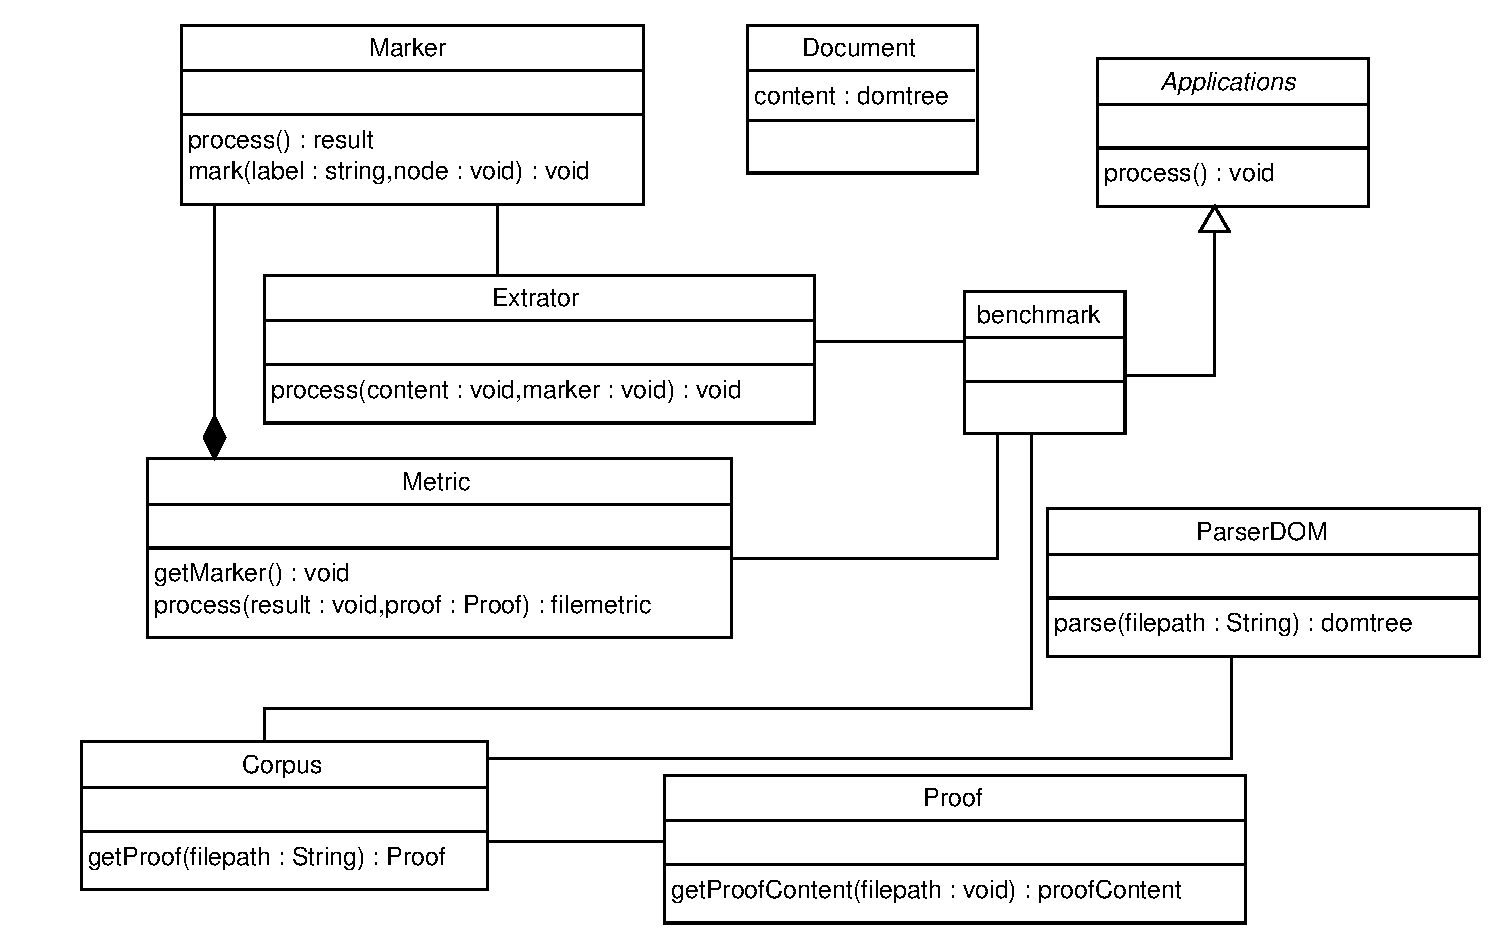
\includegraphics[width=12cm]{img/classes.eps}
%  \caption{x}
%  \label{x}
%  \end{center}
%\end{figure}

% Le esse paragrafo de novo. Tah faltando pontuacao.

% \balancecolumns

\bibliographystyle{alpha}
\bibliography{bib}
\end{document}
